\chapter{Klassediagram}
For at illustrere modellaget i vore MVC-mønster, har vi produceret et klassediagram i UML, der simplificerer strukturen. 
Det skal bemærkes, at klasserne og felterne er på dansk i diagrammet, og på engelsk i selve koden af programmet.
\section{Klasserne}
Vi vil gennemgå klasserne, der optræder i klassediagrammet, og beskrive deres relatoner samt de felter de indeholder. Ydermere vil deres rolle i programmet opsumeres tilsidst.
\subsection{Person}
Person-klassen i modellen, er den der holder styr på brugeren og dennes basale atributter - herunder brugernavn, kodeord og kaldenavn. 
Ydermere er det vigtigt, at objektet kan indeholde informationer om personens madpræferencer og vurderinger af opskrifter; Dette er med til at give person-klassen en mere intim vinket, og så at sige bedre afspejle den virkelige person, samt fungere som grundlag for anbefaling af opskrifter. 
Det er naturligvis også vigtigt for et program, der omhandler bl.a. indkøbslister, at holde styr på en persons indkøbslister og lignende. 
Til dette har person-klassen to felter der hedder henholdsvis, grupper og indkøbslister. 
Begge felter er lister, der holder styr på personens relationer til netop grupper og indkøbslister - En person kan altså have relationer til flere grupper og flere indkøbslister, hvilket også kan ses ud fra de indtegnede relationer i klassediagrammet.
\subsection{Grupper} 
\begin{figure}[h]
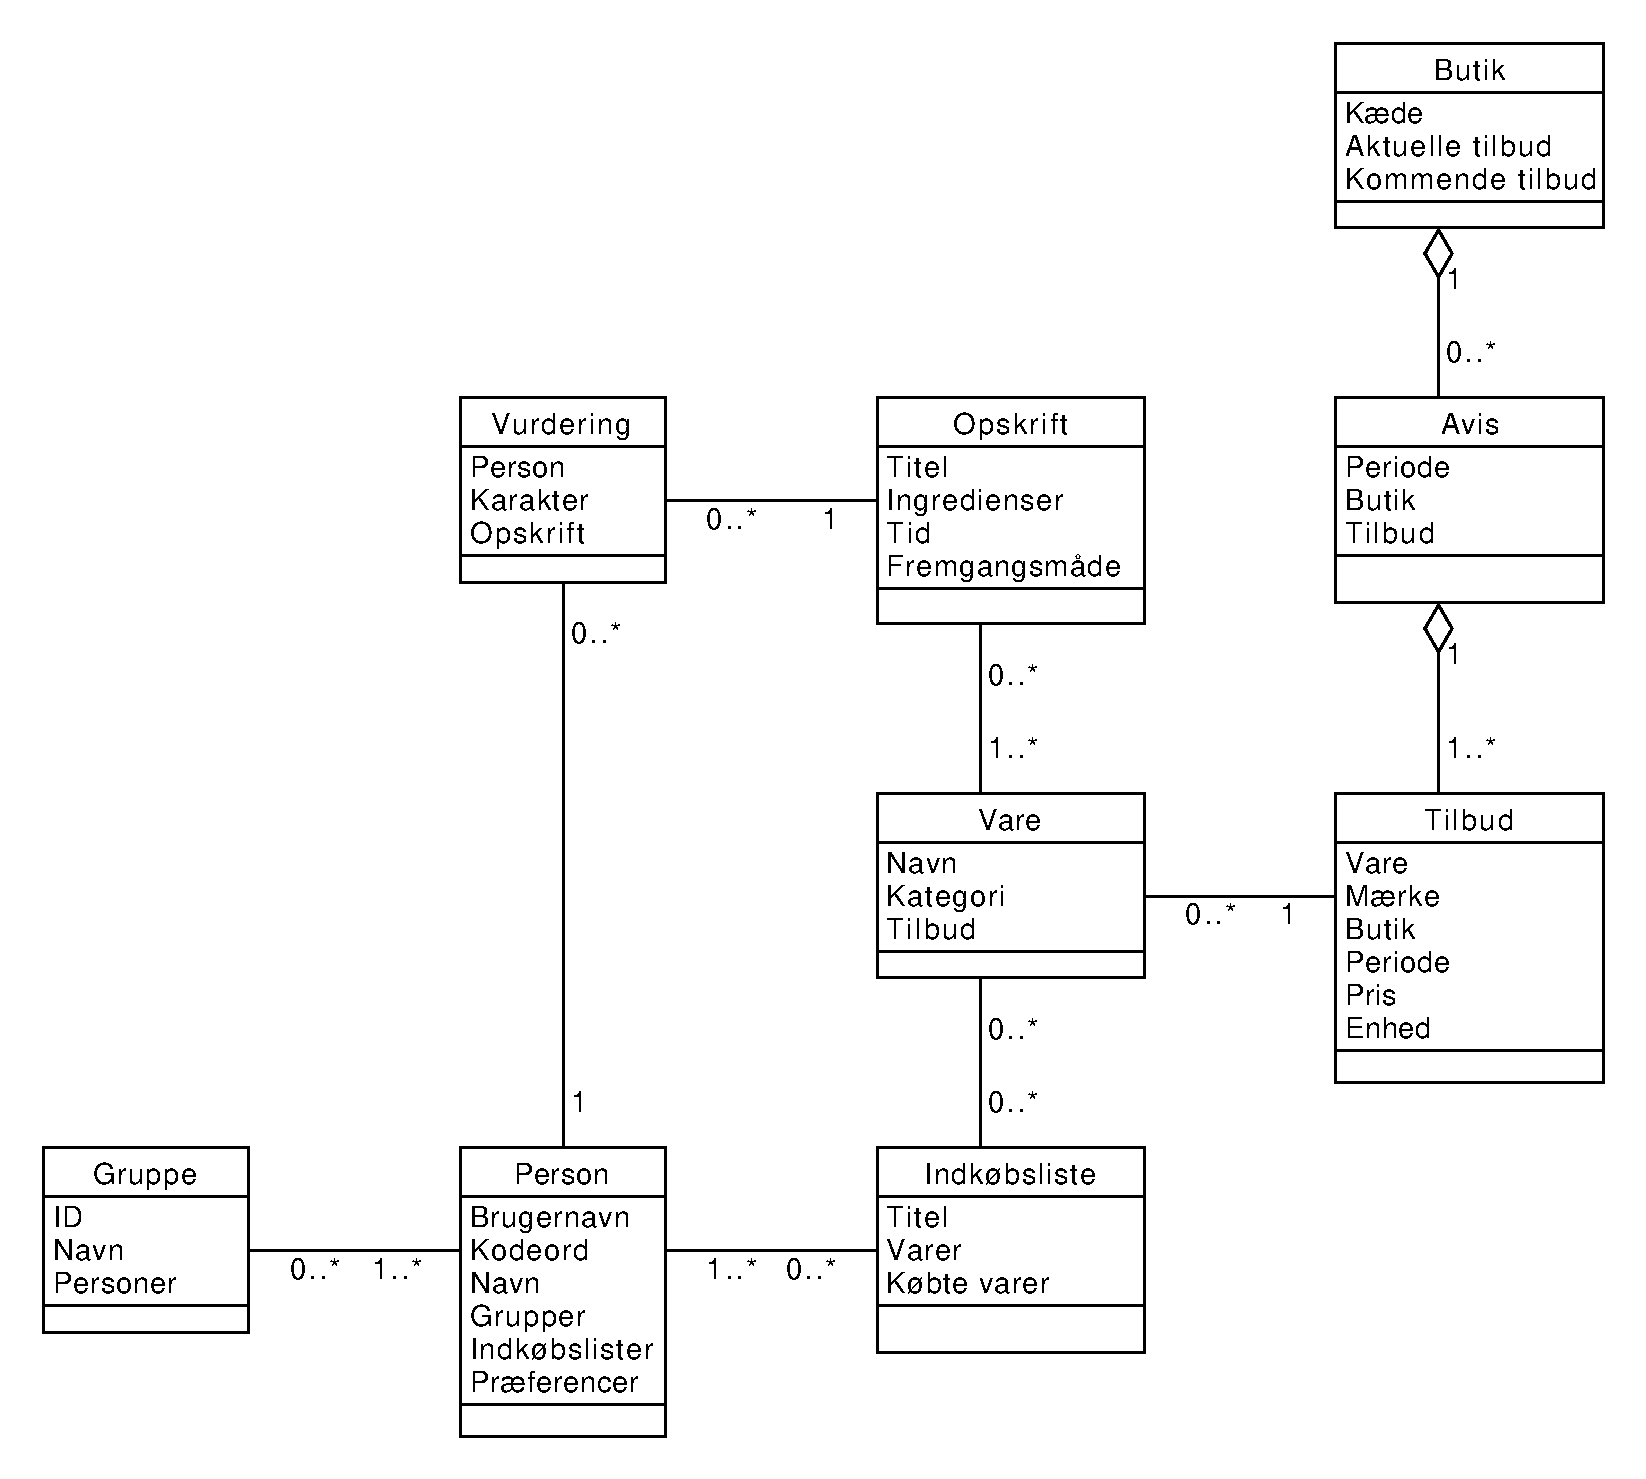
\includegraphics[width=\linewidth]{/Diagrams/klassediagram_model_expanded_implemented.pdf}
\caption{UML klassediagram for modellaget i MVC-mønsteret}
\end{figure}
